\begin{frame}{Problem considered} 
	\textbf{Problem statement:} Consider the Poisson problem in 3D with Dirichlet BC:
	\vspace{-5pt}
	\begin{equation*}
		\left\{
		\begin{aligned}
			-\Delta u & = f, \; &  & \text{in } \; \Omega \times \mathcal{M}, \\
			u         & =0, \;  &  & \text{on } \; \partial\Omega \times \mathcal{M},
		\end{aligned}
		\right.
		% \label{eq:Lap2D}\tag{$\mathcal{P}$}
	\end{equation*}

	\vspace{-5pt}
	with $\Omega=[-0.5 \pi, 0.5 \pi]^3$ and $\mathcal{M}=[-0.5,0.5]^3$ ($p=3$ parameters).
		
	\vspace{8pt}
	\textbf{Analytical solution:} $\bm{\mu}=(\mu_1,\mu_2,\mu_3) \in \mathcal{M}$

	\vspace{-5pt}
	\begin{equation*}
		% \label{eq:analytical_solution_Lap2D}
		u(\bm{x},\bm{\mu})=\exp\left(-\frac{{(x-\mu_1)}^2+{(y-\mu_2)}^2+{(z-\mu_3)}^2}{2}\right)\sin(2x)\sin(2y)\sin(2z).
	\end{equation*}

	\vspace{12pt}
	\textbf{PINN training:} \\
	MLP 5 layers (tanh - 40, 60, 60, 60, 40); LBFGs optimizer (5000 epochs - 40000 col. pts). \\
	Imposing the Dirichlet BC exactly in the PINN with the levelset $\varphi$ defined by
	$$\varphi(\bm{x})=(x+0.5\pi)(x-0.5\pi)(y+0.5\pi)(y-0.5\pi)(z+0.5\pi)(z-0.5\pi).$$
	
	\small
	Training time: 12 minutes on NVIDIA RTX 2000 (8GB VRAM).
\end{frame}

\begin{frame}{Online phase - 1 parameters instance I}
	\vspace{-12pt}
	$$\bm{\mu}^{(1)}=(0.05, 0.22, 0.1) $$
	% \vspace{2pt}

	\begin{minipage}[t]{0.4\linewidth}
		\textbf{Error estimates in $L^2$ norm:}
		\vspace{-10pt}
		\begin{figure}[H]
			\only<1-2>{\cvgFEMCorrOnedeg{images/numeric/Poisson3DDirichlet/cvg/FEM_case1_v2_param1_degree1.csv}{images/numeric/Poisson3DDirichlet/cvg/Corr_case1_v2_param1_degree1.csv}{2e-5}{false}}
			\only<3>{\cvgFEMCorrOnedeg{images/numeric/Poisson3DDirichlet/cvg/FEM_case1_v2_param1_degree1.csv}{images/numeric/Poisson3DDirichlet/cvg/Corr_case1_v2_param1_degree1.csv}{2e-5}{true}}
		\end{figure}
	\end{minipage} \hspace{1cm}
	\begin{minipage}[t]{0.5\linewidth}
		\only<2-3>{
			\textbf{$L^2$ error w.r.t. execution time$^*$:}
			\vspace{-14pt}
			\begin{figure}[H]
				\only<2>{
					\cvgtimeerror{images/numeric/Poisson3DDirichlet/time_error/FEM_case1_v2_param1_degree1_time_error.csv}{images/numeric/Poisson3DDirichlet/time_error/Corr_case1_v2_param1_degree1_time_error.csv}{false}
				}
				\only<3>{
					\cvgtimeerror{images/numeric/Poisson3DDirichlet/time_error/FEM_case1_v2_param1_degree1_time_error.csv}{images/numeric/Poisson3DDirichlet/time_error/Corr_case1_v2_param1_degree1_time_error.csv}{true}
				}
			\end{figure}
			\vspace{-20pt}

			$^*$ mesh + assembly + solve \\
			\textcolor{addcolor}{\; + prior derivatives evaluation} \\
			\textcolor{addcolor}{\; \sout{+ training time}}	}
	\end{minipage}
\end{frame}

\begin{frame}{Online phase - 1 parameters instance II}
	\vspace{-12pt}
	$$\bm{\mu}^{(1)}=(0.05, 0.22, 0.1) $$

	\textbf{$N_\text{dofs}$ and computation time required to reach the same error $e$:}

	\begin{table}[ht!]
		\centering
		\timerequired{images/numeric/Poisson3DDirichlet/timerequired/TabTimes_case1_v2_param1_degree1.csv}
	\end{table}
	\hspace{240pt}\begin{tikzpicture}
		\flechecourbehorizontale{2.5}{0.1}{2}{-0.2}{$\div 1471$}{darkred}
	\end{tikzpicture}

	Cartesian mesh: $N^3$ nodes; $\mathbb{P}_1$ elements.

	\vfill
	\footnotesize
	$^*$ The results in brackets are extrapolations.

\end{frame}

\begin{frame}{Parametric framework}
	\textbf{How many parameters instance $n_p$ are needed to balance training?}

	\vspace{-5pt}
	\begin{figure}[H]
		\hspace{-15pt}\begin{minipage}[t]{0.43\linewidth}
			\centering
			\cvgtimeerrorparam{images/numeric/Poisson3DDirichlet/parametric_framework/output13.csv}
		\end{minipage} \hspace{20pt}
		\begin{minipage}[t]{0.49\linewidth}
			\centering
			\cvgtimeerrorparamD{images/numeric/Poisson3DDirichlet/parametric_framework/output54.csv}
		\end{minipage}
	\end{figure}

	\vspace{-15pt}
	\hspace{50pt} To achieve $e=10^{-3}$ \hspace{75pt} To achieve $e=5\cdot 10^{-4}$

	\vspace{10pt}
	\textbf{Online:} assembly + solve \textcolor{addcolor}{\; + prior derivatives evaluation} \\

	\textbf{Offline:} mesh	\textcolor{addcolor}{\; + training time}
\end{frame}